The next step is to get a sense of the distribution of movies data set in terms of the audience score (response variable) as grouped by various levels of the relevant categorical variables. By doing this step in the Exploratory Data Analysis process, we cannot only get a sense of important trends of the data, but also being able to get a sense of the relationship between the response variable and categorical predictor variables. Specifically, we could gauge the sign of slope coefficient for each categorical predictor variable as well as the potential statistical significance of those predictors in predicting the response variable. This step can be done by constructing boxplots for the audience score as grouped by the selected categorical variables.

\begin{figure}[htbp]
\begin{center}
\caption{Boxplots of Audience Score vs. Genre, and Audience Score v.s MPAA Rating}
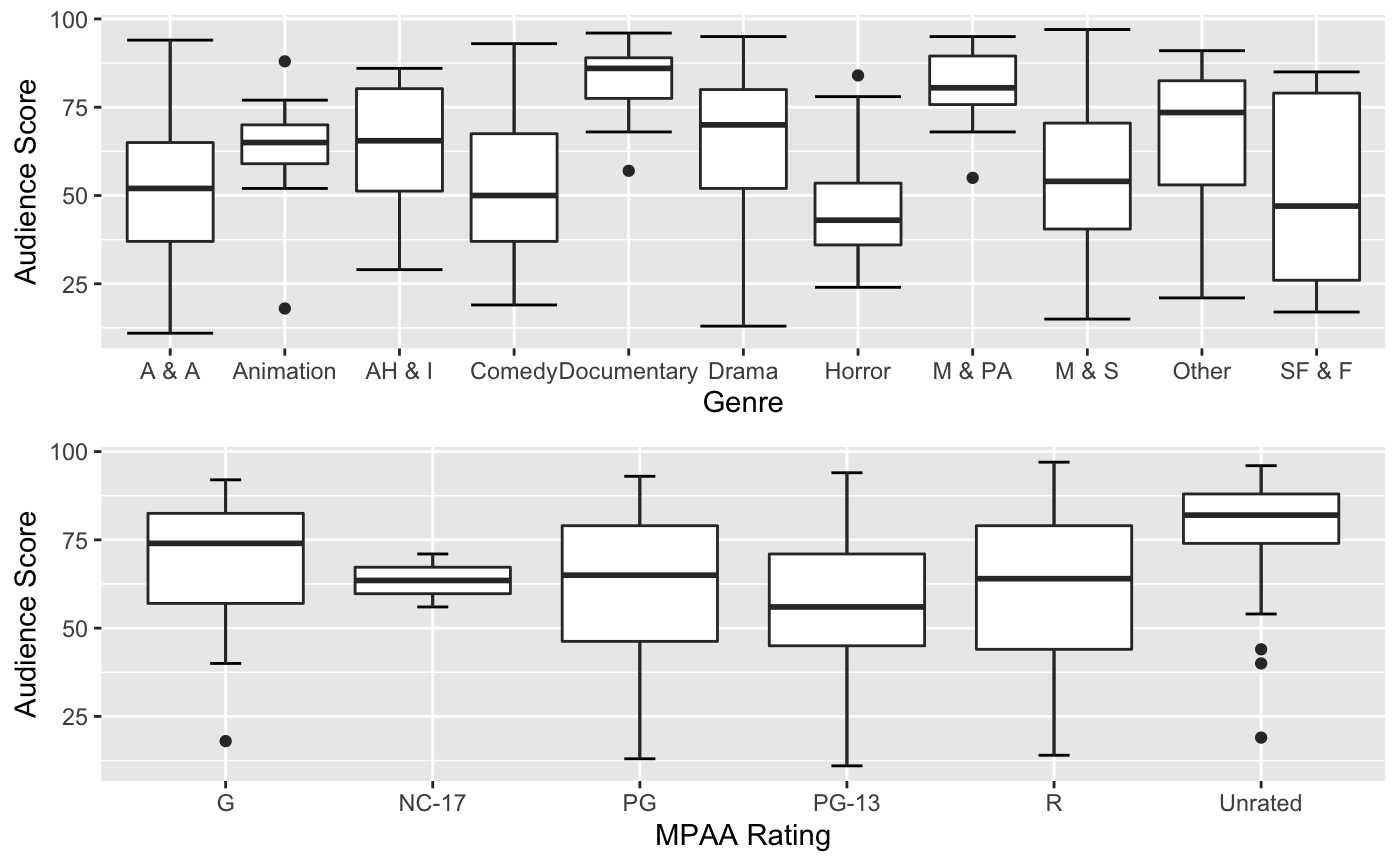
\includegraphics[scale=0.32]{boxplot1.png}
\label{fig: 7}
\end{center}
\end{figure}

According to Figure~\ref{fig: 7}, movies with genres, such as Documentary, Drama, Musical 
and Performing Arts tend to have higher audience scores, while movies with Horror genre are 
less popular. In terms of MPAA Rating, movies that are unrated expect to have higher audience scores, while movies rated as 'PG-13' seem to have lower audience scores.

The boxplot (Figure~\ref{fig: 8} upper left) depicting the distribution of audience score by whether or not the movie received an Oscar Best Picture Nomination conveys the fact that movies that receive a Best Picture Nomination tend to have a higher audience score in comparison to those movies that have not received such nomination. Similarly, the boxplot (Figure~\ref{fig: 8} upper right) depicting the distribution of audience score by whether or not the movie won an Oscar Best Picture Award coveys the similar fact that movies that won a Best Picture Award tend to have a higher audience score in comparison to those movies that have not won a Best Picture Award. For movies not won a Best Picture Award, the distribution of the audience score is fairly symmetric since the median is somewhat located near the center of the box. Nevertheless, the distribution of audience score for movies that won a Best Picture has a right-skewed distribution since the longer part of the box is above the median, indicating that Best Picture Winning movies are likely to receive audience scores higher than the median level. Moreover, there is a potential outlier in this category with audience score  69 but does received a Best Picture Award. 

The boxplot (Figure~\ref{fig: 8} lower left) depicting the distribution of audience score by whether or not the movie is included in the Top 200 Box Office indicates the fact that movies that were included in this list tend to receive a higher audience score compared to movies that were not included in this list. For movies that were not included in the Top 200 Box Office list, the distribution of the audience score is fairly symmetric due to the fact that the median is located near the center of the box. On the contrary, the distribution of audience scores for movies that were included in the list seems skewed to the left as the longer part of the box is below the median. This means that movies feature in the Top 200 Box Office list are likely to receive lower audience scores compared to the median level.

\begin{figure}[htbp]
\begin{center}
\caption{Boxplots of Audience Score vs. Oscar Best Picture Nomination, Audience Score vs. Oscar Best Picture Win, Audience Score vs. Top 200 Box Office List, and Audience Score vs. Audience Rating}
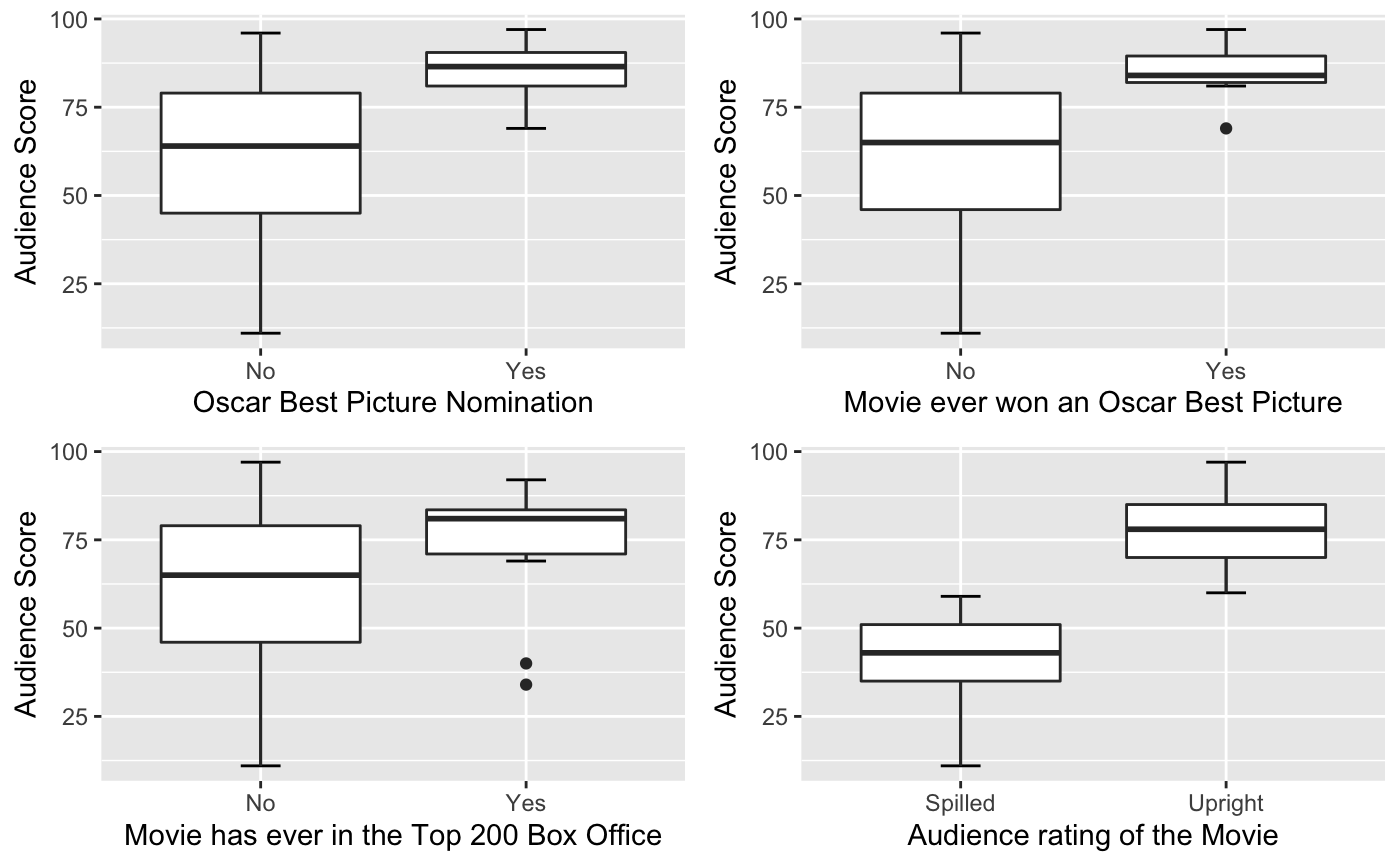
\includegraphics[scale=0.32]{boxplot2.png}
\label{fig: 8}
\end{center}
\end{figure}

The boxplot (Figure~\ref{fig: 8} lower right) depicting the distribution of audience score by the audience rating that the movie received on Rotten Tomatoes. Based on this plot, it seems movies that received an "Upright" audience rating on Rotten Tomatoes tend to receive higher audience scores in comparison to movies that received a "Spilled" audience rating. Moreover, the box of movies that received an "Upright" audience rating on Rotten Tomatoes is completely above the box of movies that received a "Spilled" audience rating. This indicates that there is a significant difference between those two groups and it is highly possible that audience rating could be a good predictor variable of the audience score.

Figure~\ref{fig: 9} includes another four boxplots of the distribution of audience score as grouped by another four categorical predictor variables. To sum up, there seems to be no significant difference between the distributions of audience score grouped by whether or not the actors of movies ever won an Oscar, as well as whether or not the actresses of the movies ever won an Oscar. This may indicates that those two categorical variables may not be a good predictor variable for the audience score (Two Sample T-Test show P-value greater than 0.05). In addition, there seems to be little difference between the distribution of audience score grouped by whether or not movie director has ever won an Oscar, but the difference is very small (although it passed the Two Sample T-Test with a P-value = 0.01617). This difference indicates that movies that have a director who won an Oscar at least once during his or here career seem to receive higher audience score in comparison to movies that have a director who has never won an Oscar. I am going to keep those variables and the model selection process will decide which variables will be selected into the model anyway.

\begin{figure}[htbp]
\begin{center}
\caption{Boxplots of Audience Score vs. Best Actor Win, Audience Score vs. Best Actress Win, Audience Score vs. Best Director Win, Audience Score vs. Type of the Movie}
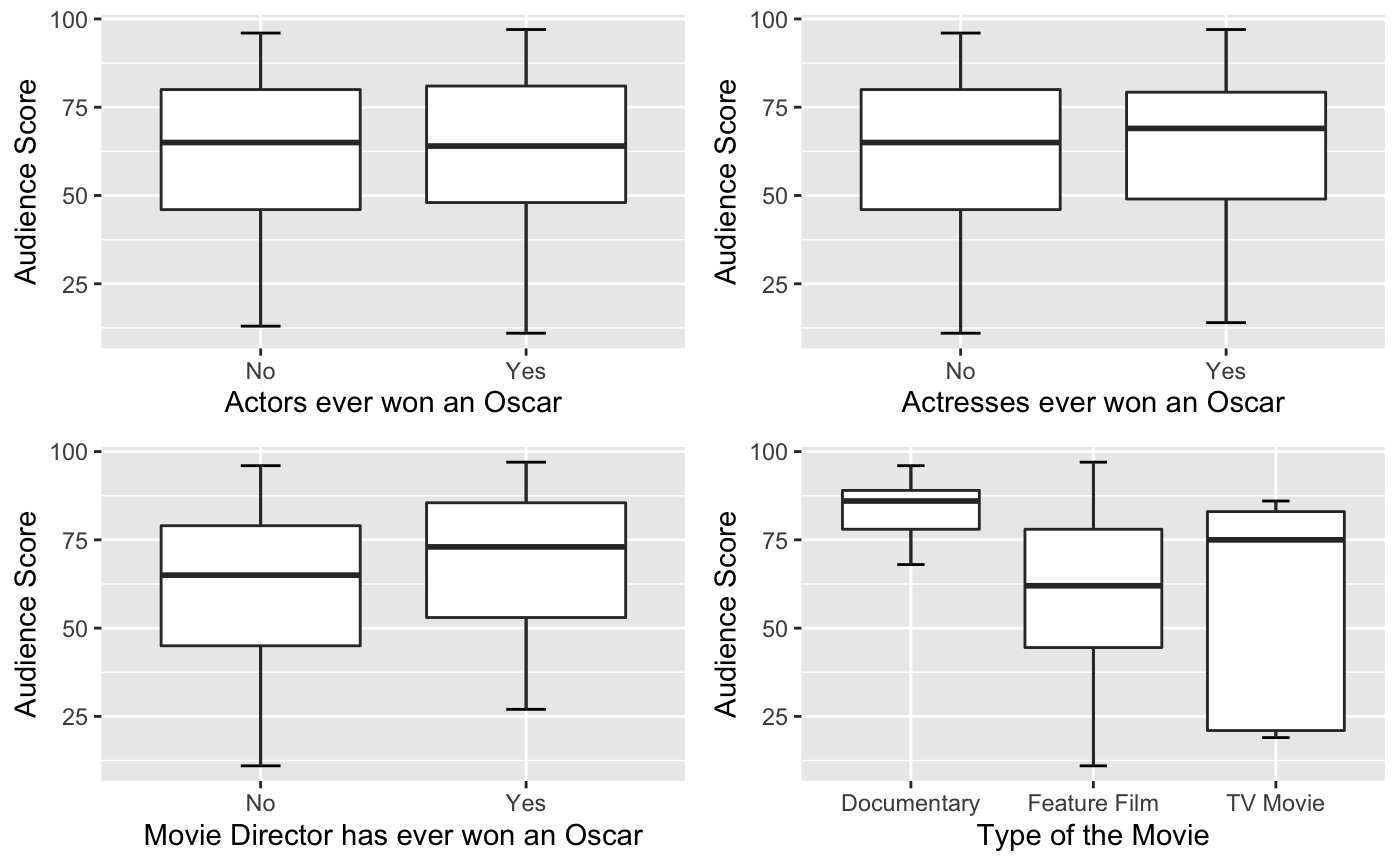
\includegraphics[scale=0.32]{boxplot3.png}
\label{fig: 9}
\end{center}
\end{figure}

The boxplot (Figure~\ref{fig: 9} lower right) depicting the distribution of the audience score by movie type (Documentary, Feature Film, and TV Movie) indicates that Documentary tend to receive higher audience scores in comparison to Feature Film and TV Movies. Moreover, the distribution of audience score by Feature Film is fairly symmetric, but the distribution of audience score for both Documentary and TV Movie is skewed to the left, which indicates that the majority of audience scores for Documentary and TV Movie are lying below the median level. 

\begin{figure}[htbp]
\begin{center}
\caption{Boxplot of Audience Score vs. Critics Rating of the Movie}
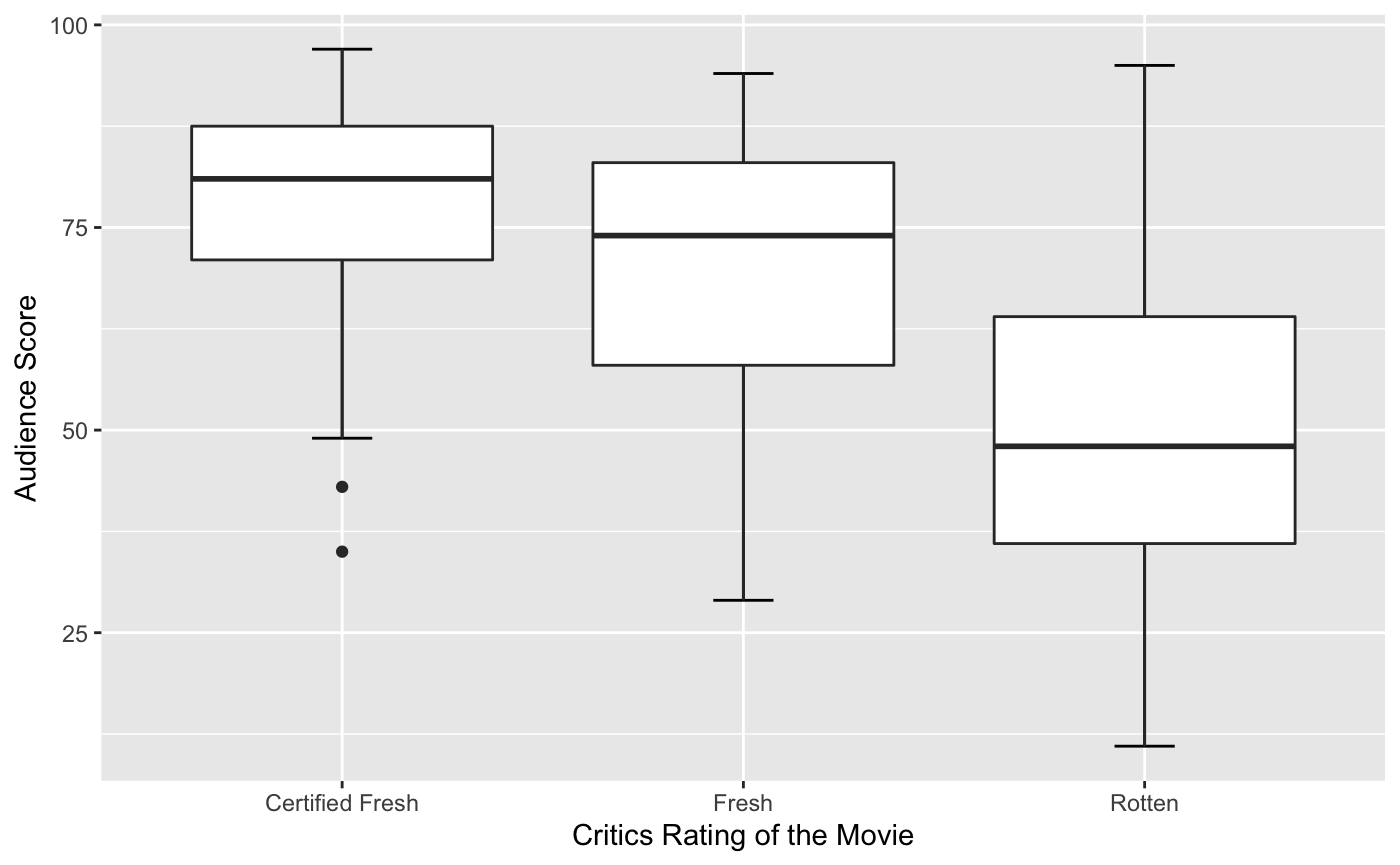
\includegraphics[scale=0.32]{boxplot4.png}
\label{fig: 10}
\end{center}
\end{figure}

The last boxplot (Figure~\ref{fig: 10}) depicting the distribution of the audience score by three levels of critics rating on Rotten Tomatoes, which are "Certified Fresh", "Fresh" and "Rotten". The plot tends to show that movies that receive a "Certified Fresh" seem to receive higher audience score compared to movies that received a "Fresh" or "Rotten". The distribution of audience score for movies received either "Certified Fresh" or "Fresh" are skewed to the left, indicating that the majority of audience scores are lying below the median level, while movies received "Rotten" seems to be skewed to the right. The difference between movies with either a "Certified Fresh" or a "Fresh" on critics rating and movies with a "Rotten" critics rating in terms of mean audience score is quite significant (as shown in Two-Sample T-Test). To be specific, the audience score fall into the bottom 25\% of movies with "Certified Fresh" critics rating is somewhat higher than the mean and median audience score of movies with "Rotten" critics rating. Therefore, the critics rating on Rotten Tomatoes may also be a good predictor for movie's audience score.

In the next section, I am going to perform the model selection to decide what variables should be kept in the model.

